\clearpage
\cleardoublepage

\chapter{Training Process and Frameworks}

\section{Introduction}

Training a neural network is the process of finding a set of parameters that minimize a given loss function over a dataset. While the mathematical foundations of optimization (gradient descent, backpropagation) were covered in previous chapters, this chapter focuses on the \emph{practical and theoretical aspects} of the training process itself. We examine why certain techniques work, how to diagnose training failures, and what modern frameworks provide to make large-scale training tractable.

The training process encompasses several interrelated components: the optimization algorithm, the regularization strategy, the hyperparameter configuration, and the infrastructure for efficient computation. A deep understanding of how these components interact is essential for successfully training modern neural networks.

\section{The Training Loop}

Neural network training consists of iterative optimization over data using minibatch stochastic gradient descent (SGD) or its variants.

\subsection{Formal Description}

Given a dataset $\mathcal{D} = \{(\mathbf{x}_i, \mathbf{y}_i)\}_{i=1}^{N}$, a model $f(\mathbf{x}; \theta)$ with parameters $\theta$, and a loss function $\ell$, the training objective is:
\begin{equation}
\theta^* = \arg\min_{\theta} \frac{1}{N}\sum_{i=1}^{N} \ell\bigl(f(\mathbf{x}_i; \theta), \mathbf{y}_i\bigr)
\end{equation}

In practice, we compute the gradient over minibatches $\mathcal{B}_t \subset \mathcal{D}$ of size $B$:
\begin{equation}
\mathbf{g}_t = \nabla_\theta \frac{1}{B}\sum_{i \in \mathcal{B}_t} \ell\bigl(f(\mathbf{x}_i; \theta_t), \mathbf{y}_i\bigr)
\end{equation}

\begin{algorithm}[H]
\caption{Training Loop}
\begin{enumerate}
    \item Initialize model weights $\theta_0$
    \item For each epoch $e = 1, 2, \ldots, E$:
    \begin{enumerate}
        \item Shuffle training data
        \item For each minibatch $\mathcal{B}_t$:
        \begin{enumerate}
            \item Forward pass: compute predictions $\hat{\mathbf{y}} = f(\mathbf{x}; \theta_t)$
            \item Compute loss $\mathcal{L}_t = \frac{1}{B}\sum_{i \in \mathcal{B}_t} \ell(\hat{\mathbf{y}}_i, \mathbf{y}_i)$
            \item Backward pass: compute gradients $\mathbf{g}_t = \nabla_\theta \mathcal{L}_t$
            \item Update weights: $\theta_{t+1} = \theta_t - \alpha \cdot \text{optimizer\_step}(\mathbf{g}_t)$
        \end{enumerate}
        \item Evaluate on validation set
        \item Save checkpoint if validation metric improved
    \end{enumerate}
    \item Return best model
\end{enumerate}
\end{algorithm}

\subsection{Why Minibatch SGD Works}

A natural question is: why use small batches instead of computing the exact gradient over the full dataset? The answer lies in a beneficial interplay between three factors:

\begin{enumerate}
    \item \textbf{Noise as implicit regularization.} The gradient noise from small batches prevents the optimizer from settling into sharp minima that generalize poorly. Keskar et al.\ \cite{keskar2017largebatch} showed that large-batch training tends to converge to ``sharp'' minima with worse generalization, while small-batch SGD finds ``flat'' minima.
    
    \item \textbf{Computational efficiency.} Modern hardware (GPUs/TPUs) is optimized for parallel matrix operations. A batch size of 32--256 fully utilizes GPU parallelism while still providing meaningful gradient estimates.
    
    \item \textbf{Regular progress monitoring.} Each minibatch step provides a signal, allowing early detection of training issues (divergence, oscillation) before wasting hours of compute.
\end{enumerate}

\begin{theorem}[Convergence of SGD with Decreasing Learning Rate]
Under convexity and smoothness assumptions on $\mathcal{L}$, SGD with learning rate schedule $\alpha_t = \mathcal{O}(1/\sqrt{t})$ satisfies:
\begin{equation}
\mathbb{E}[\mathcal{L}(\theta_T)] - \mathcal{L}(\theta^*) \leq \mathcal{O}\!\left(\frac{1}{\sqrt{T}}\right)
\end{equation}
compared to $\mathcal{O}(1/T)$ for full-batch gradient descent. The slower rate is the price paid for cheaper per-step computation.
\end{theorem}

\section{Hyperparameters}

Critical hyperparameters that affect training dynamics and final model quality.

\subsection{Learning Rate}

The learning rate $\alpha$ is arguably the single most important hyperparameter. It directly controls the step size in parameter space and determines whether training converges, oscillates, or diverges.

\subsubsection{Effect of Learning Rate}

\begin{itemize}
    \item \textbf{Too high:} The loss diverges or oscillates wildly. The optimizer ``overshoots'' minima.
    \item \textbf{Too low:} Training converges extremely slowly and may get trapped in poor local minima or saddle points.
    \item \textbf{Just right:} The loss decreases steadily, with slight oscillation that provides regularization.
    \item \textbf{Typical range:} $10^{-5}$ to $0.1$
    \item \textbf{Default for Adam:} $10^{-3}$
    \item \textbf{Default for SGD:} $10^{-2}$
\end{itemize}

\subsubsection{Learning Rate Range Test}

Smith \cite{smith2017cyclical} proposed a simple but effective method for finding a good learning rate. The idea is to start with a very small learning rate and increase it exponentially during a single training run, plotting the loss against the learning rate:

\begin{enumerate}
    \item Start with $\alpha_{\min} = 10^{-6}$ (or smaller)
    \item Increase $\alpha$ by a factor of $e$ (or a constant factor) each batch
    \item Stop when the loss starts to increase
    \item Choose $\alpha$ at the point of steepest descent (typically $10^{-1}$ to $10^{-1}$ of the maximum value)
\end{enumerate}

\begin{figure}[htbp]
    \centering
    \begin{tikzpicture}[scale=0.9]
        \draw[->] (0,0) -- (10,0) node[right] {Learning rate ($\log$ scale)};
        \draw[->] (0,0) -- (0,5) node[above] {Loss};
        % Loss curve
        \draw[thick, blue] plot[smooth] coordinates {
            (0.5, 4.5) (1, 3.8) (1.5, 3.0) (2, 2.3) (2.5, 1.8) 
            (3, 1.5) (3.5, 1.3) (4, 1.2) (4.5, 1.15) (5, 1.1)
            (5.5, 1.2) (6, 1.5) (6.5, 2.0) (7, 3.0) (7.5, 4.5)
        };
        % Steepest descent point
        \draw[dashed, red] (4, 1.2) -- (4, 0) node[below] {\small $\alpha^*$};
        \draw[dashed, red] (4, 1.2) -- (0, 1.2);
        \draw[->, red, thick] (1.5, 3.0) -- (2.3, 2.2);
        \node[red, right] at (2.3, 2.5) {\small Steepest descent};
        % Labels
        \node[blue, right] at (7.5, 4.5) {\small Divergence};
        \node at (-0.3, 5) {\small High};
        \node at (-0.3, 0) {\small Low};
    \end{tikzpicture}
    \caption[Learning rate range test]{Learning rate range test. The steepest descent point $\alpha^*$ provides a good starting learning rate.}
    \label{fig:lr_range_test}
\end{figure}

\subsubsection{Learning Rate Warmup}

For large models trained with Adam, it is standard practice to use a warmup phase where the learning rate is gradually increased from zero to the target value over the first few hundred or thousand steps. This prevents instability in the early stages when the Adam momentum estimates are unreliable (being initialized to zero).

The warmup schedule is typically:
\begin{equation}
\alpha_t = \alpha_{\max} \cdot \min\!\left(1, \frac{t}{T_{\text{warmup}}}\right)
\end{equation}
where $T_{\text{warmup}}$ is the number of warmup steps (e.g., 1000 for Transformer models \cite{vaswani2017attention}).

\subsection{Batch Size}

The batch size $B$ controls how many samples are processed before each parameter update. It has profound effects on both training speed and model quality.

\subsubsection{Batch Size Effects}

\begin{itemize}
    \item \textbf{Small batch (16--64):} Noisier gradients provide implicit regularization, often better generalization. But underutilizes GPU parallelism.
    \item \textbf{Medium batch (64--256):} Good trade-off between generalization and hardware utilization. Most practitioners' default.
    \item \textbf{Large batch (256--8192+):} Better hardware utilization, faster wall-clock training. But typically requires learning rate scaling and may hurt generalization.
\end{itemize}

\subsubsection{Linear Scaling Rule}

Goyal et al.\ \cite{goyal2017accurate} proposed the linear scaling rule for large-batch training: when the batch size is multiplied by $k$, the learning rate should also be multiplied by $k$:
\begin{equation}
\alpha_{\text{large}} = \alpha_{\text{small}} \times \frac{B_{\text{large}}}{B_{\text{small}}}
\end{equation}

\begin{note}[Batch Size vs.\ Generalization]
Research by Keskar et al.\ \cite{keskar2017largebatch} and Hoffer et al.\ \cite{hoffer2017train} shows that smaller batches often achieve better generalization because gradient noise acts as implicit regularization. However, the effect depends on other factors like learning rate, network architecture, and training duration.
\end{note}

\begin{table}[ht]
    \centering
    \caption{Hyperparameter Ranges and Default Values}
    \begin{tabular}{L{2.8cm} L{3cm} L{3.5cm} L{3cm}}
        \toprule
        \textbf{Hyperparameter} & \textbf{Typical Range} & \textbf{Default} & \textbf{Notes} \\
        \midrule
        Learning Rate & $10^{-5}$ to $0.1$ & Adam: $10^{-3}$; SGD: $10^{-2}$ & Most important \\
        Batch Size & 16--8192 & 32--256 & Depends on GPU memory \\
        Epochs & 10--1000 & Task-dependent & Early stopping recommended \\
        Weight Decay & $10^{-6}$ to $10^{-2}$ & $10^{-2}$ (AdamW) & See Section~\ref{sec:weight_decay} \\
        Dropout Rate & 0.1--0.5 & 0.1--0.3 & See Section~\ref{sec:dropout_theory} \\
        Momentum & 0.9--0.999 & 0.9 (SGD) & 0.9/0.999 for Adam \\
        Warmup Steps & 0--10K & 1000 (Transformers) & Large models benefit more \\
        \bottomrule
    \end{tabular}
\end{table}

\section{Regularization}

Regularization encompasses all techniques that reduce overfitting by constraining the model's capacity or adding noise to the training process. We provide theoretical foundations for the most important methods.

\subsection{Dropout}
\label{sec:dropout_theory}

Dropout \cite{srivastava2014dropout} is a regularization technique that randomly sets neuron activations to zero during training with probability $p$ (the dropout rate).

\subsubsection{Forward Pass with Dropout}

During training, for a layer with input $\mathbf{x}$ and weight matrix $\mathbf{W}$:
\begin{equation}
\mathbf{y} = \mathbf{W} \cdot (\mathbf{x} \odot \mathbf{m}), \quad \mathbf{m} \sim \text{Bernoulli}(1 - p)
\end{equation}
where $\mathbf{m}$ is a binary mask and $\odot$ denotes element-wise multiplication.

\subsubsection{Inverted Dropout}

The standard implementation uses \emph{inverted dropout}, which scales activations during training so that no scaling is needed at inference time:
\begin{equation}
\mathbf{y} = \frac{\mathbf{W} \cdot (\mathbf{x} \odot \mathbf{m})}{1 - p}
\end{equation}

This ensures that $\mathbb{E}[\mathbf{y}_{\text{train}}] = \mathbf{W}\mathbf{x} = \mathbf{y}_{\text{inference}}$, meaning the expected output is the same with and without dropout.

\textbf{Proof:} For any component $x_j$ of the input:
\begin{align}
\mathbb{E}\left[\frac{x_j \cdot m_j}{1 - p}\right] &= \frac{1}{1-p} \cdot \mathbb{E}[x_j \cdot m_j] \\
&= \frac{1}{1-p} \cdot x_j \cdot \mathbb{E}[m_j] \\
&= \frac{1}{1-p} \cdot x_j \cdot (1 - p) = x_j
\end{align}

\subsubsection{Ensemble Interpretation}

Dropout can be understood as training an ensemble of $2^n$ sub-networks (where $n$ is the number of dropout units) that share parameters. Each forward pass with a different mask effectively samples a different sub-network. At inference time, all sub-networks are averaged (which, by the linearity of the scaling, is equivalent to using the full network).

More precisely, a network with $n$ dropout units has $2^n$ possible thinned networks. The dropout training objective minimizes:
\begin{equation}
\mathcal{L}_{\text{dropout}} = \mathbb{E}_{\mathbf{m} \sim \text{Bernoulli}(1-p)} \left[\ell\bigl(f(\mathbf{x}; \theta \odot \mathbf{m}), \mathbf{y}\bigr)\right]
\end{equation}

This is equivalent to minimizing a \emph{bagged ensemble} objective, which explains dropout's regularization effect through variance reduction.

\subsubsection{Dropout as Approximate Bayesian Inference}

Gal and Ghahramani \cite{gal2016dropout} showed that dropout in a neural network is mathematically equivalent to approximate variational inference in a deep Gaussian process. Under this interpretation:
\begin{itemize}
    \item Each dropout mask defines a sample from an approximate posterior $q(\theta)$
    \item The KL divergence between the approximate and true posterior is minimized implicitly
    \item Multiple stochastic forward passes at inference provide uncertainty estimates
\end{itemize}

This provides a principled explanation for why dropout provides not just regularization but also \emph{model uncertainty} estimates---a crucial property for safety-critical applications.

\subsubsection{Dropout Variants}

\begin{table}[ht]
    \centering
    \caption{Dropout Variants and Their Properties}
    \begin{tabular}{L{3cm} L{4cm} L{4cm}}
        \toprule
        \textbf{Variant} & \textbf{Mechanism} & \textbf{Use Case} \\
        \midrule
        Standard Dropout & Randomly zero activations & Fully connected layers \\
        Spatial Dropout & Drop entire feature maps & Convolutional layers \\
        DropConnect & Randomly zero weights & Alternative to dropout \\
        DropBlock & Drop contiguous regions & Convolutional layers \\
        Attention Dropout & Drop attention weights & Transformer models \\
        Feature Dropout & Drop input features & Input regularization \\
        \bottomrule
    \end{tabular}
\end{table}

\subsection{Weight Decay}
\label{sec:weight_decay}

\subsubsection{L2 Regularization as MAP Estimation}

Weight decay (L2 regularization) adds a penalty on the magnitude of model parameters:
\begin{equation}
\mathcal{L}_{\text{reg}} = \mathcal{L} + \frac{\lambda}{2}\|\mathbf{W}\|_F^2
\end{equation}

This has a elegant interpretation as \emph{maximum a posteriori} (MAP) estimation. Assume a Gaussian prior on the weights $\mathbf{W} \sim \mathcal{N}(0, \sigma_w^2 \mathbf{I})$. The MAP objective is:
\begin{align}
\theta_{\text{MAP}} &= \arg\max_\theta \log p(\mathcal{D} | \theta) + \log p(\theta) \\
&= \arg\min_\theta \underbrace{-\sum_{i=1}^N \log p(\mathbf{y}_i | \mathbf{x}_i, \theta)}_{\mathcal{L}} + \underbrace{\frac{1}{2\sigma_w^2}\|\mathbf{W}\|_F^2}_{\lambda/2 \cdot \|\mathbf{W}\|_F^2}
\end{align}

Thus, L2 regularization with coefficient $\lambda$ is equivalent to MAP estimation with a Gaussian weight prior of variance $\sigma_w^2 = 1/\lambda$.

\subsubsection{Weight Decay vs.\ L2 Regularization: AdamW}

For adaptive optimizers like Adam, there is a subtle but important difference between L2 regularization and decoupled weight decay. In standard Adam with L2 regularization, the weight update becomes:
\begin{equation}
\mathbf{W}_{t+1} = \mathbf{W}_t - \alpha \cdot \frac{\hat{\mathbf{m}}_t}{\sqrt{\hat{\mathbf{v}}_t} + \epsilon} \odot \left(\nabla \mathcal{L}_t + \lambda \mathbf{W}_t\right)
\end{equation}

The problem is that the weight decay term $\lambda \mathbf{W}_t$ is scaled by the adaptive learning rate $\frac{1}{\sqrt{\hat{\mathbf{v}}_t} + \epsilon}$, meaning parameters with large historical gradients receive \emph{less} regularization---the opposite of what we want.

Loshchilov and Hutter \cite{loshchilov2019decoupled} proposed \textbf{AdamW}, which decouples weight decay from the gradient-based update:
\begin{align}
\mathbf{W}_{t+1} &= \mathbf{W}_t - \alpha \cdot \frac{\hat{\mathbf{m}}_t}{\sqrt{\hat{\mathbf{v}}_t} + \epsilon} \odot \nabla \mathcal{L}_t - \alpha\lambda \mathbf{W}_t \\
&= (1 - \alpha\lambda)\mathbf{W}_t - \alpha \cdot \frac{\hat{\mathbf{m}}_t}{\sqrt{\hat{\mathbf{v}}_t} + \epsilon} \odot \nabla \mathcal{L}_t
\end{align}

This ensures that weight decay is applied uniformly regardless of the adaptive learning rate, leading to significantly better generalization in practice.

\subsection{Other Regularization Techniques}

\subsubsection{Gradient Clipping}

For training very deep networks or recurrent networks, gradients can become extremely large, causing parameter updates that destabilize training. Gradient clipping limits the gradient norm:
\begin{equation}
\text{If } \|\mathbf{g}\| > c: \quad \mathbf{g} \leftarrow \frac{c}{\|\mathbf{g}\|}\mathbf{g}
\end{equation}

where $c$ is a threshold (commonly 1.0 or 5.0 for Transformer models). Pascanu et al.\ \cite{pascanu2013difficulty} showed that gradient clipping is essential for training RNNs on long sequences.

\subsubsection{Label Smoothing}

Label smoothing \cite{szegedy2016rethinking} replaces hard one-hot labels with a softer distribution. Instead of target $\mathbf{y} = [0, \ldots, 0, 1, 0, \ldots, 0]$, we use:
\begin{equation}
y_k^{\text{smooth}} = (1 - \epsilon)\cdot y_k + \frac{\epsilon}{K}
\end{equation}
where $\epsilon$ is the smoothing coefficient (typically 0.1) and $K$ is the number of classes.

\textbf{Why label smoothing works:} It prevents the model from becoming overconfident. A model that outputs $p(\text{correct}) = 0.999$ on training data is likely memorizing rather than learning. Label smoothing penalizes this by requiring the model to distribute some probability mass to incorrect classes, which:
\begin{itemize}
    \item Improves calibration (predicted probabilities better reflect true accuracy)
    \item Acts as implicit regularization; \cite{muller2019when} connects it to adding KL divergence between the output distribution and a uniform prior
    \item Improves BLEU scores in machine translation by 0.5--1.0
\end{itemize}

\subsubsection{Stochastic Depth}

Huang et al.\ \cite{huang2016deep} proposed randomly dropping entire residual blocks during training (analogous to dropout but at the block level). This allows training very deep networks (e.g., 1200 layers) by reducing effective depth during training:
\begin{equation}
\mathbf{y} = \begin{cases} \mathcal{F}_l(\mathbf{x}) + \mathbf{x} & \text{with probability } p_l \\ \mathbf{x} & \text{with probability } 1 - p_l \end{cases}
\end{equation}
where $p_l$ is the survival probability for layer $l$, often following a linear decay schedule from the first to the last layer.

\section{Early Stopping}

Early stopping halts training when validation performance stops improving. Despite its simplicity, it is one of the most effective and widely used regularization techniques.

\subsection{Algorithm}

\begin{enumerate}
    \item Monitor validation loss (or a suitable metric) at the end of each epoch
    \item Save the model checkpoint whenever the validation metric improves
    \item If no improvement is observed for $N$ epochs (the \emph{patience}), stop training
    \item Return the best checkpoint (not the final one)
\end{enumerate}

Typical patience values: 10--20 epochs for small models, 5--10 epochs for large models.

\subsection{Early Stopping as Regularization}

Yao et al.\ showed that early stopping provides regularization effects equivalent to weight decay under certain conditions. The intuition is clear:

\begin{enumerate}
    \item A model at epoch $t$ has parameters $\theta_t$ that lie along the optimization trajectory
    \item As training progresses, the model fits increasingly fine-grained patterns in the training data
    \item Beyond a certain point, these patterns are noise (overfitting)
    \item Early stopping selects parameters from the ``sweet spot'' where the model has learned signal but not noise
\end{enumerate}

Formally, for gradient descent on a linear model with quadratic loss, early stopping is equivalent to Tikhonov regularization (L2 weight decay), with the number of gradient steps playing the role of the regularization strength.

\section{Backpropagation}

\subsection{The Computational Graph Perspective}

Backpropagation is the algorithm for efficiently computing gradients through a computational graph by applying the chain rule in reverse topological order. While the mathematical principle is straightforward---the chain rule---the computational efficiency comes from reusing intermediate results.

\subsubsection{Forward Pass}

Consider a simple computation: $z = f(g(x))$. The forward pass computes:
\begin{align}
a &= g(x) \\
z &= f(a)
\end{align}

\subsubsection{Backward Pass}

The backward pass computes gradients in reverse order:
\begin{align}
\frac{\partial \mathcal{L}}{\partial a} &= \frac{\partial \mathcal{L}}{\partial z} \cdot \frac{\partial z}{\partial a} = \frac{\partial \mathcal{L}}{\partial z} \cdot f'(a) \\
\frac{\partial \mathcal{L}}{\partial x} &= \frac{\partial \mathcal{L}}{\partial a} \cdot \frac{\partial a}{\partial x} = \frac{\partial \mathcal{L}}{\partial a} \cdot g'(x)
\end{align}

\subsection{Example: Two-Layer Network}

For a two-layer network with loss $\mathcal{L}$:
\begin{align}
\mathbf{h} &= \sigma(\mathbf{W}_1 \mathbf{x} + \mathbf{b}_1) \\
\hat{\mathbf{y}} &= \mathbf{W}_2 \mathbf{h} + \mathbf{b}_2 \\
\mathcal{L} &= \ell(\hat{\mathbf{y}}, \mathbf{y})
\end{align}

\begin{figure}[htbp]
    \centering
    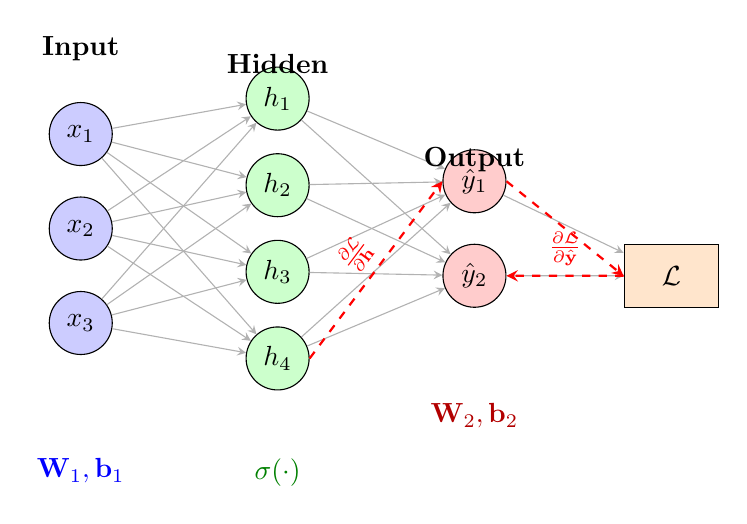
\begin{tikzpicture}[
        node distance=1.5cm,
        neuron/.style={circle, draw, minimum size=8mm, inner sep=0pt},
        >=stealth
    ]
        % Input layer
        \foreach \i in {1,2,3} {
            \node[neuron, fill=blue!20] (I\i) at (0, -\i*1.2+2.4) {$x_{\i}$};
        }
        % Hidden layer
        \foreach \j in {1,2,3,4} {
            \node[neuron, fill=green!20] (H\j) at (2.5, -\j*1.1+2.75) {$h_{\j}$};
        }
        % Output layer
        \foreach \k in {1,2} {
            \node[neuron, fill=red!20] (O\k) at (5, -\k*1.2+1.8) {$\hat{y}_{\k}$};
        }
        % Loss
        \node[rectangle, draw, fill=orange!20, minimum width=1.2cm, minimum height=8mm] (L) at (7.5, -0.6) {$\mathcal{L}$};
        
        % Forward connections
        \foreach \i in {1,2,3} {
            \foreach \j in {1,2,3,4} {
                \draw[->, thin, gray!60] (I\i) -- (H\j);
            }
        }
        \foreach \j in {1,2,3,4} {
            \foreach \k in {1,2} {
                \draw[->, thin, gray!60] (H\j) -- (O\k);
            }
        }
        \foreach \k in {1,2} {
            \draw[->, thin, gray!60] (O\k) -- (L);
        }
        
        % Backward gradient arrows (red, dashed)
        \draw[->, thick, red, dashed] (L.west) -- node[above, font=\small] {$\frac{\partial \mathcal{L}}{\partial \hat{\mathbf{y}}}$} (O2.east);
        \draw[->, thick, red, dashed] (O1.east) -- (L.west);
        \draw[->, thick, red, dashed] (H4.east) -- node[above, font=\small, sloped] {$\frac{\partial \mathcal{L}}{\partial \mathbf{h}}$} (O1.west);
        
        % Labels
        \node[above] at (0, 2.0) {\textbf{Input}};
        \node[above] at (2.5, 1.85) {\textbf{Hidden}};
        \node[above] at (5, 0.6) {\textbf{Output}};
        
        % Layer labels
        \node[below, blue] at (0, -2.8) {$\mathbf{W}_1, \mathbf{b}_1$};
        \node[below, green!50!black] at (2.5, -2.8) {$\sigma(\cdot)$};
        \node[below, red!70!black] at (5, -2.1) {$\mathbf{W}_2, \mathbf{b}_2$};
    \end{tikzpicture}
    \caption{Computational graph for a two-layer network. Solid arrows represent forward computation; dashed red arrows represent backward gradient flow.}
    \label{fig:computational_graph}
\end{figure}

The backward pass computes:
\begin{align}
\frac{\partial \mathcal{L}}{\partial \hat{\mathbf{y}}} &= \nabla_{\hat{\mathbf{y}}} \ell \\
\frac{\partial \mathcal{L}}{\partial \mathbf{W}_2} &= \frac{\partial \mathcal{L}}{\partial \hat{\mathbf{y}}} \mathbf{h}^\top, \qquad \frac{\partial \mathcal{L}}{\partial \mathbf{b}_2} = \frac{\partial \mathcal{L}}{\partial \hat{\mathbf{y}}} \\
\frac{\partial \mathcal{L}}{\partial \mathbf{h}} &= \mathbf{W}_2^\top \frac{\partial \mathcal{L}}{\partial \hat{\mathbf{y}}} \\
\frac{\partial \mathcal{L}}{\partial \mathbf{a}} &= \frac{\partial \mathcal{L}}{\partial \mathbf{h}} \odot \sigma'(\mathbf{a}) \\
\frac{\partial \mathcal{L}}{\partial \mathbf{W}_1} &= \frac{\partial \mathcal{L}}{\partial \mathbf{a}} \mathbf{x}^\top, \qquad \frac{\partial \mathcal{L}}{\partial \mathbf{b}_1} = \frac{\partial \mathcal{L}}{\partial \mathbf{a}}
\end{align}
where $\mathbf{a} = \mathbf{W}_1 \mathbf{x} + \mathbf{b}_1$ is the pre-activation.

\subsection{Automatic Differentiation}

Modern deep learning frameworks implement \emph{reverse-mode automatic differentiation} (autodiff), which is distinct from both numerical differentiation and symbolic differentiation:

\begin{table}[ht]
    \centering
    \caption{Comparison of Differentiation Methods}
    \begin{tabular}{L{3cm} L{3.5cm} L{3.5cm} L{3cm}}
        \toprule
        \textbf{Method} & \textbf{Accuracy} & \textbf{Speed} & \textbf{Usage} \\
        \midrule
        Numerical & Approximate & Slow ($n$ evaluations) & Debugging only \\
        Symbolic & Exact & Fast but memory-heavy & CAS (Mathematica) \\
        Reverse autodiff & Exact (to machine $\epsilon$) & $\mathcal{O}(1)\times$ forward pass & PyTorch, JAX \\
        \bottomrule
    \end{tabular}
\end{table}

The key insight of reverse-mode autodiff is that computing \emph{all} partial derivatives of a scalar-valued function with respect to $n$ inputs costs only $\mathcal{O}(1)$ times the cost of the forward pass, regardless of $n$. This makes it ideal for neural networks, where the loss is scalar but there are millions of parameters.

\subsection{Common Training Pitfalls}

\begin{table}[ht]
    \centering
    \caption{Diagnosing Training Failures}
    \begin{tabular}{L{4cm} L{5cm} L{4.5cm}}
        \toprule
        \textbf{Symptom} & \textbf{Likely Cause} & \textbf{Solution} \\
        \midrule
        Loss doesn't decrease & Learning rate too low & Increase LR or check data \\
        Loss is NaN & Learning rate too high & Decrease LR, add grad clipping \\
        Train loss decreases, val loss increases & Overfitting & Add regularization, early stopping \\
        Loss oscillates & Batch size too small & Increase batch size or decrease LR \\
        Very slow convergence & Learning rate too low & Use LR finder \\
        Gradients vanish & Deep network, bad init & Use residual connections, ReLU \\
        \bottomrule
    \end{tabular}
\end{table}

\section{Model Checkpointing}

Saving and restoring model state during training is essential for long-running experiments and production deployment.

\begin{itemize}
    \item \textbf{Model architecture:} The network definition (layer sizes, types)
    \item \textbf{Weights:} The learned parameters $\theta$
    \item \textbf{Optimizer state:} Momentum terms $\mathbf{m}$, adaptive learning rates $\mathbf{v}$ (required to resume training exactly)
    \item \textbf{Epoch and step counters:} Training progress
    \item \textbf{Best metric:} The validation metric for model selection
    \item \textbf{Random state:} RNG seed for reproducibility
\end{itemize}

\section{Mixed Precision Training}

\subsection{Motivation}

Standard training uses 32-bit floating point (FP32) for all computations. Mixed precision training uses 16-bit floating point (FP16) for most operations while maintaining a 32-bit master copy of weights, achieving:
\begin{itemize}
    \item \textbf{2$\times$ memory reduction:} Activations and gradients stored in FP16
    \item \textbf{2--3$\times$ speedup:} Modern GPUs have 2$\times$ FP16 throughput vs FP32 (Tensor Cores on NVIDIA GPUs provide up to 8$\times$ for FP16 matmul)
    \item \textbf{No accuracy loss:} When implemented correctly with loss scaling
\end{itemize}

\subsection{The Loss Scaling Problem}

FP16 has a limited dynamic range ($\approx 6 \times 10^{-5}$ to $65504$). Gradients smaller than $2^{-24}$ underflow to zero. Since gradients in deep networks can span many orders of magnitude, small gradients may be lost entirely.

\textbf{Solution:} Scale the loss by a factor $S$ before backpropagation, then unscale the gradients before the optimizer step:
\begin{align}
\hat{\mathcal{L}} &= S \cdot \mathcal{L} \\
\mathbf{g}_{\text{FP32}} &= \frac{1}{S} \cdot \nabla_{\theta_{\text{FP16}}} \hat{\mathcal{L}}
\end{align}

Dynamic loss scaling \cite{micikevicius2018mixed} automatically adjusts $S$: increase $S$ by a factor of 2 every $N$ successful steps, and halve $S$ whenever gradients overflow (contain NaN/Inf).

\subsection{BF16: The Modern Alternative}

Bfloat16 (BF16) uses the same 8 exponent bits as FP32 but only 7 mantissa bits (vs.\ 10 for FP16). This gives BF16 the same dynamic range as FP32 ($\approx 10^{-38}$ to $10^{38}$), eliminating the need for loss scaling entirely. BF16 is supported on NVIDIA A100/H100 GPUs and is becoming the default for training large language models.

\begin{table}[ht]
    \centering
    \caption{Floating Point Format Comparison}
    \begin{tabular}{L{2.5cm} M{1.5cm} M{1.5cm} M{1.5cm} M{3cm}}
        \toprule
        \textbf{Property} & \textbf{FP32} & \textbf{FP16} & \textbf{BF16} & \textbf{TF32} \\
        \midrule
        Total bits & 32 & 16 & 16 & 19 \\
        Exponent bits & 8 & 5 & 8 & 8 \\
        Mantissa bits & 23 & 10 & 7 & 10 \\
        Dynamic range & $\pm 3.4 \times 10^{38}$ & $\pm 65504$ & $\pm 3.4 \times 10^{38}$ & $\pm 3.4 \times 10^{38}$ \\
        Loss scaling needed & No & Yes & No & No \\
        Hardware support & Universal & Tensor Cores & A100+ & A100+ \\
        \bottomrule
    \end{tabular}
\end{table}

\section{PyTorch Framework}

PyTorch is the most popular framework for deep learning research due to its eager execution model and Pythonic API.

\begin{code}
    \captionof{listing}{Complete Training Loop in PyTorch}
    \label{code:training_pytorch}
\begin{lstlisting}[language=python]
import torch
import torch.nn as nn
import torch.optim as optim
from torch.utils.data import DataLoader

# Model definition
model = nn.Sequential(
    nn.Linear(784, 512),
    nn.BatchNorm1d(512),
    nn.GELU(),
    nn.Dropout(0.2),
    nn.Linear(512, 256),
    nn.BatchNorm1d(256),
    nn.GELU(),
    nn.Dropout(0.1),
    nn.Linear(256, 10)
)

# Loss, optimizer, and scheduler
criterion = nn.CrossEntropyLoss(label_smoothing=0.1)
optimizer = optim.AdamW(model.parameters(), lr=1e-3, 
                        weight_decay=0.01)
scheduler = optim.lr_scheduler.CosineAnnealingLR(
    optimizer, T_max=100, eta_min=1e-5)

# Training loop with mixed precision
scaler = torch.cuda.amp.GradScaler()
device = torch.device('cuda' if torch.cuda.is_available() 
                      else 'cpu')
model = model.to(device)

best_val_loss = float('inf')
patience = 10
patience_counter = 0

for epoch in range(num_epochs):
    # --- Training ---
    model.train()
    train_loss = 0.0
    for data, target in train_loader:
        data, target = data.to(device), target.to(device)
        
        optimizer.zero_grad(set_to_none=True)
        
        # Mixed precision forward pass
        with torch.cuda.amp.autocast():
            output = model(data.view(data.size(0), -1))
            loss = criterion(output, target)
        
        scaler.scale(loss).backward()
        scaler.unscale_(optimizer)
        torch.nn.utils.clip_grad_norm_(model.parameters(), max_norm=1.0)
        scaler.step(optimizer)
        scaler.update()
        
        train_loss += loss.item()
    
    scheduler.step()
    
    # --- Validation ---
    model.eval()
    val_loss = 0.0
    correct = 0
    with torch.no_grad():
        for data, target in val_loader:
            data, target = data.to(device), target.to(device)
            with torch.cuda.amp.autocast():
                output = model(data.view(data.size(0), -1))
                val_loss += criterion(output, target).item()
            pred = output.argmax(dim=1)
            correct += pred.eq(target).sum().item()
    
    val_acc = 100. * correct / len(val_loader.dataset)
    avg_val_loss = val_loss / len(val_loader)
    
    # --- Checkpointing with early stopping ---
    if avg_val_loss < best_val_loss:
        best_val_loss = avg_val_loss
        patience_counter = 0
        torch.save({
            'epoch': epoch,
            'model_state_dict': model.state_dict(),
            'optimizer_state_dict': optimizer.state_dict(),
            'best_val_loss': best_val_loss,
        }, 'best_model.pt')
    else:
        patience_counter += 1
        if patience_counter >= patience:
            print(f'Early stopping at epoch {epoch}')
            break
\end{lstlisting}
\end{code}

\section{CUDA and GPU Training}

\subsection{GPU Programming Model}

GPUs excel at data-parallel operations through thousands of lightweight cores organized into streaming multiprocessors (SMs). Key considerations for efficient GPU utilization:

\begin{itemize}
    \item \textbf{Data transfer:} CPU--GPU transfers (PCIe) are orders of magnitude slower than GPU computation. Minimize transfers by keeping data on GPU.
    \item \textbf{Kernel launch overhead:} Many small operations are slower than fewer large operations. Use fused kernels when possible.
    \item \textbf{Memory coalescing:} Adjacent threads should access adjacent memory addresses for optimal bandwidth.
    \item \textbf{Occupancy:} The ratio of active threads to maximum threads affects utilization but is not the only factor.
\end{itemize}

\subsection{Distributed Training}

For models too large for a single GPU, distributed training strategies are essential:

\begin{table}[ht]
    \centering
    \caption{Distributed Training Strategies}
    \begin{tabular}{L{3cm} L{4cm} L{3cm} L{3cm}}
        \toprule
        \textbf{Strategy} & \textbf{Mechanism} & \textbf{Memory} & \textbf{Speed} \\
        \midrule
        Data Parallel & Replicate model, split data & Linear in model & Near-linear scale \\
        Model Parallel & Split model across GPUs & Reduced & Communication-bound \\
        Pipeline Parallel & Split layers across GPUs & Reduced & Bubble overhead \\
        Tensor Parallel & Split tensors within a layer & Reduced & All-reduce cost \\
        FSDP & Shard parameters + gradients & Reduced & Communication cost \\
        \bottomrule
    \end{tabular}
\end{table}

\subsection{Gradient Accumulation}

When the desired effective batch size exceeds GPU memory, gradient accumulation simulates larger batches by accumulating gradients over multiple micro-batches before each optimizer step:
\begin{equation}
\mathbf{g} = \frac{1}{K}\sum_{k=1}^{K} \nabla_\theta \mathcal{L}(\mathcal{B}_k)
\end{equation}
where $K$ is the number of accumulation steps and the effective batch size is $B_{\text{eff}} = B \times K$.

\begin{code}
    \captionof{listing}{Gradient Accumulation in PyTorch}
    \label{code:grad_accum}
\begin{lstlisting}[language=python]
accumulation_steps = 4  # Effective batch = 32 * 4 = 128
optimizer.zero_grad()

for i, (data, target) in enumerate(train_loader):
    output = model(data)
    loss = criterion(output, target) / accumulation_steps
    loss.backward()  # Accumulate gradients
    
    if (i + 1) % accumulation_steps == 0:
        optimizer.step()
        optimizer.zero_grad()
\end{lstlisting}
\end{code}

\section{Training Diagnostics}

Understanding what happens during training requires systematic monitoring of several indicators.

\subsection{Loss Curves}

\begin{figure}[htbp]
    \centering
    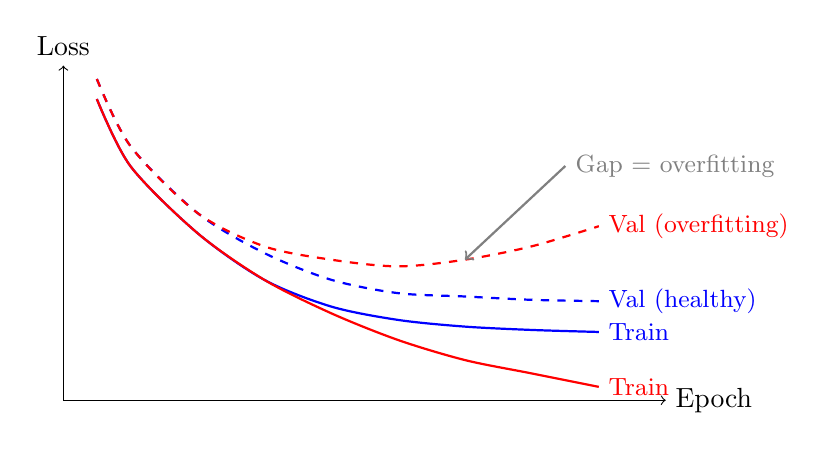
\begin{tikzpicture}[scale=0.85]
        \draw[->] (0,0) -- (9,0) node[right] {Epoch};
        \draw[->] (0,0) -- (0,5) node[above] {Loss};
        
        % Healthy training
        \draw[thick, blue] plot[smooth] coordinates {
            (0.5, 4.5) (1, 3.5) (2, 2.5) (3, 1.8) (4, 1.4) 
            (5, 1.2) (6, 1.1) (7, 1.05) (8, 1.02)
        };
        % Healthy validation
        \draw[thick, blue, dashed] plot[smooth] coordinates {
            (0.5, 4.8) (1, 3.8) (2, 2.8) (3, 2.2) (4, 1.8) 
            (5, 1.6) (6, 1.55) (7, 1.5) (8, 1.48)
        };
        
        % Overfitting
        \draw[thick, red] plot[smooth] coordinates {
            (0.5, 4.5) (1, 3.5) (2, 2.5) (3, 1.8) (4, 1.3) 
            (5, 0.9) (6, 0.6) (7, 0.4) (8, 0.2)
        };
        % Overfitting validation
        \draw[thick, red, dashed] plot[smooth] coordinates {
            (0.5, 4.8) (1, 3.8) (2, 2.8) (3, 2.3) (4, 2.1) 
            (5, 2.0) (6, 2.1) (7, 2.3) (8, 2.6)
        };
        
        % Legend
        \node[blue, right] at (8, 1.02) {\small Train};
        \node[blue, right] at (8, 1.48) {\small Val (healthy)};
        \node[red, right] at (8, 0.2) {\small Train};
        \node[red, right] at (8, 2.6) {\small Val (overfitting)};
        
        % Annotation
        \draw[<-, thick, gray] (6, 2.1) -- (7.5, 3.5) node[right, font=\small] {Gap = overfitting};
    \end{tikzpicture}
    \caption{Training loss curves: healthy training (blue) vs.\ overfitting (red). Solid lines: training loss. Dashed lines: validation loss.}
    \label{fig:training_curves}
\end{figure}

\subsection{Gradient Statistics}

Monitoring gradient statistics helps diagnose training issues:
\begin{itemize}
    \item \textbf{Gradient norm:} Should be stable. Spikes indicate instability; vanishing norm indicates dead neurons or saturated activations.
    \item \textbf{Gradient distribution:} Should be approximately Gaussian. Heavy tails may indicate outlier samples.
    \item \textbf{Update-to-weight ratio:} The ratio $\|\alpha \mathbf{g}\| / \|\mathbf{W}\|$ should be around $10^{-3}$. Much larger values indicate instability; much smaller values indicate stagnation.
    \item \textbf{Activation statistics:} Mean and variance of layer activations should remain stable across training. BatchNorm helps with this.
\end{itemize}

\section{Chapter Summary}

\begin{enumerate}
    \item Training involves iterative minibatch optimization over data, where gradient noise provides implicit regularization
    \item The learning rate is the most critical hyperparameter; the LR range test provides a principled way to select it
    \item Warmup is essential for large models with adaptive optimizers to stabilize early training
    \item Dropout provides regularization through ensemble averaging and can be interpreted as approximate Bayesian inference
    \item AdamW decouples weight decay from adaptive learning rates, leading to better generalization than L2 regularization with Adam
    \item Early stopping prevents overfitting and is equivalent to regularization under certain conditions
    \item Mixed precision training (FP16/BF16) provides 2--3$\times$ speedup with no accuracy loss when properly implemented
    \item Gradient accumulation enables training with effective batch sizes larger than GPU memory
    \item Systematic monitoring of loss curves, gradient statistics, and validation metrics is essential for diagnosing training issues
\end{enumerate}

\section{Further Reading}

\begin{itemize}
    \item \cite{pascanu2013difficulty} --- On the Difficulty of Training Recurrent Neural Networks (Gradient Clipping)
    \item \cite{srivastava2014dropout} --- Dropout: A Simple Way to Prevent Neural Networks from Overfitting
    \item \cite{goodfellow2016deep} --- Chapter 7 (Regularization) and Chapter 8 (Optimization for Training Deep Models)
    \item \cite{gal2016dropout} --- Dropout as a Bayesian Approximation: Representing Model Uncertainty in Deep Learning
    \item \cite{huang2016deep} --- Deep Networks with Stochastic Depth (Stochastic Depth)
    \item \cite{szegedy2016rethinking} --- Rethinking the Inception Architecture for Computer Vision (Label Smoothing)
    \item \cite{goyal2017accurate} --- Accurate, Large Minibatch SGD: Training ImageNet in 1 Hour
    \item \cite{keskar2017largebatch} --- On Large-Batch Training for Deep Learning: Generalization Gap and Sharp Minima
    \item \cite{smith2017cyclical} --- Cyclical Learning Rates for Training Neural Networks (LR range test)
    \item \cite{micikevicius2018mixed} --- Mixed Precision Training
    \item \cite{loshchilov2019decoupled} --- Decoupled Weight Decay Regularization (AdamW)
    \item \cite{rajbhandari2020zero} --- ZeRO: Memory Optimizations Toward Training Trillion Parameter Models
\end{itemize}

\section{Exercises}

\begin{enumerate}
    \item \textbf{Learning-Rate Range Test:} Describe how you would run an LR range test and interpret the loss curve to choose an initial learning rate.

    \item \textbf{Warmup Rationale:} Why is warmup especially important for large-batch training and Transformer optimization? What failure mode does it prevent?

    \item \textbf{Weight Decay:} Compare L2 regularization and AdamW in the context of adaptive optimizers. Why can the two behave differently?

    \item \textbf{Early Stopping:} Explain why early stopping can be viewed as a form of regularization. What validation pattern suggests that training should stop?

    \item \textbf{Mixed Precision:} If FP16 halves activation memory, what secondary mechanism is typically added to keep gradients numerically stable?

    \item \textbf{Gradient Accumulation:} Suppose you can fit batch size 16 on one GPU but want an effective batch size of 128. How many accumulation steps are required, and what should happen to the loss before calling backward?
\end{enumerate}

